\documentclass{article}
\usepackage[margin=1in]{geometry}
\usepackage{graphicx}
\usepackage{float}
\usepackage{bm}
%\pagestyle{empty}

\title{\vspace{-2.5cm}Tabulate Equations of Common Ellipse Parameters}
\author{Dr. Elliot Grafil}

\begin{document}
\maketitle
%\thispagestyle{empty}
\section*{Introduction}
This document tabulates the equations needed to deduce any of the seven common parameters of an ellipse given two of its parameters. 
\begin{figure}[H]
\begin{center}
\noindent\makebox[\textwidth]{
  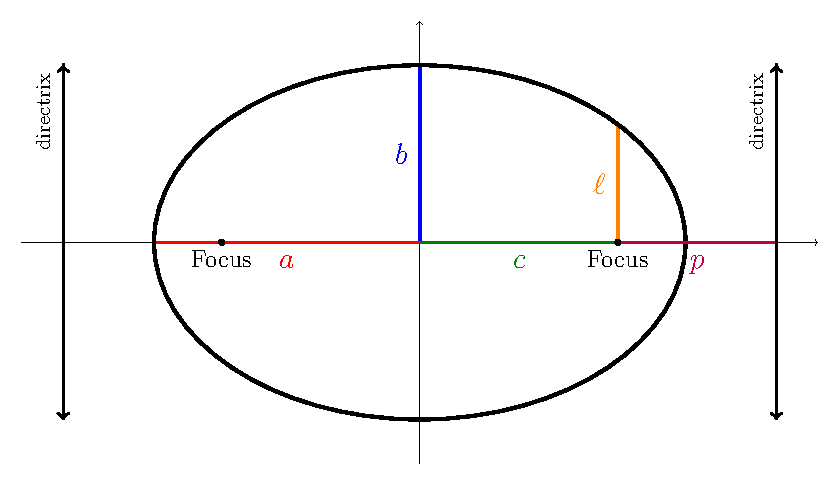
\includegraphics[scale=1.25]{./EllipseDiagram/EllipseDiagram.pdf}
  }
  \caption{Common parameters labeled on an example ellipse. Eccentricity, $e$, is not depicted.}
  \label{fig:boat1}
  \end{center}
\end{figure}
\subsection*{\centering{Parameters}}
\begin{description}
\item[$\boldsymbol{a}$] Semi-Major Axis. The length from the center of the ellipse to the farthest point on the curve.
\item[$\boldsymbol{b}$] Semi-Minor Axis. The length from the center of the ellipse to the nearest point on the curve.
\item[$\boldsymbol{c}$] Linear eccentricity. The length from the center of the ellipse to one of its foci.
\item[$\boldsymbol{e}$] Eccentricity. Measurement of deviation from being circular. Sometimes denoted as $\epsilon$. Can be confuse with flattening that shares the symbol $\epsilon$.
\item[$\boldsymbol{\ell}$] Semi-Latus Rectum. The length of a line segment that begins at the focus and makes contact with the ellipse. It is perpendicular to the major axis.
\item[$\boldsymbol{p}$] Focal parameter. The length from one of the two foci to the nearest directrix.
\item[$\boldsymbol{x}$] Directrix (distance). The distance along the major axis from the center of the ellipse at which the directrix line lies. Sometimes denoted as $d$ or $y$. In special cases it is the equation for the directrix line. 
\end{description}

\section*{Other Useful Relations \& Terminology}
\begin{description}
\item[Major Axis] Double the length of the semi-major axis ($2a$). The length of the ellipse at its widest point.
\item[Minor Axis] Double the length of the semi-minor axis ($2b$). The length of the ellipse at its thinnest point.
\item[Focal Length] Double the length of the linear eccentricity ($2e$). The length between the ellipse's two foci.
\item[Flattening] A rarer type of measurement for the deviation from being circular. Flattening is given usually in terms of $a$ and $b$ as $f=\frac{a-b}{a}$ or $e$ as $f=1-\sqrt{1-e^2}$. Sometimes denoted as $\epsilon$.
\item[Latus Rectum] Double the length of the semi-latus rectum ($2\ell$). The chord that passes through a focus and is perpendicular to the major axis.
\end{description}

\section*{How To Use}
For the parameter of interest go to the page labeled with the parameters name. 
The first row and column are labeled with different variables. 
Select a row and column based on what information you already have. 
The equation that is displayed in the intersection is the function used to derived the parameter given the two variables.    
\newpage

\section*{\centering{Semi-Major Axis}}
\begin{center}
\noindent\makebox[\textwidth]{%
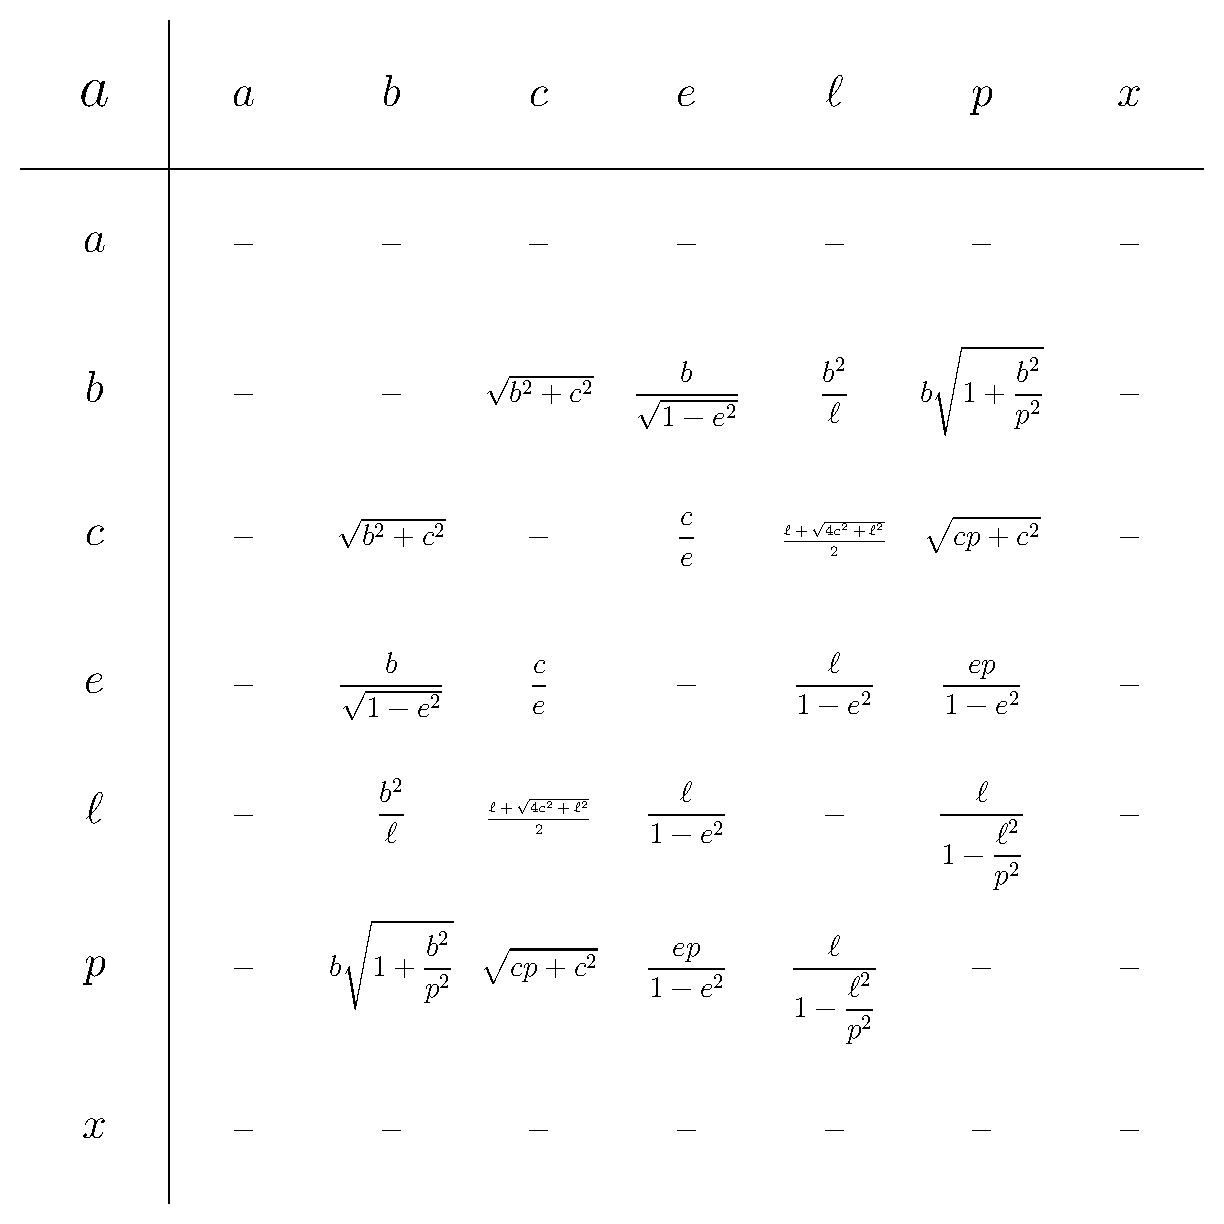
\includegraphics[scale=.95]{./AEquation/AEllipseEquations.pdf}
}
\newpage

\section*{\centering{Semi-Minor Axis}}
\noindent\makebox[\textwidth]{%
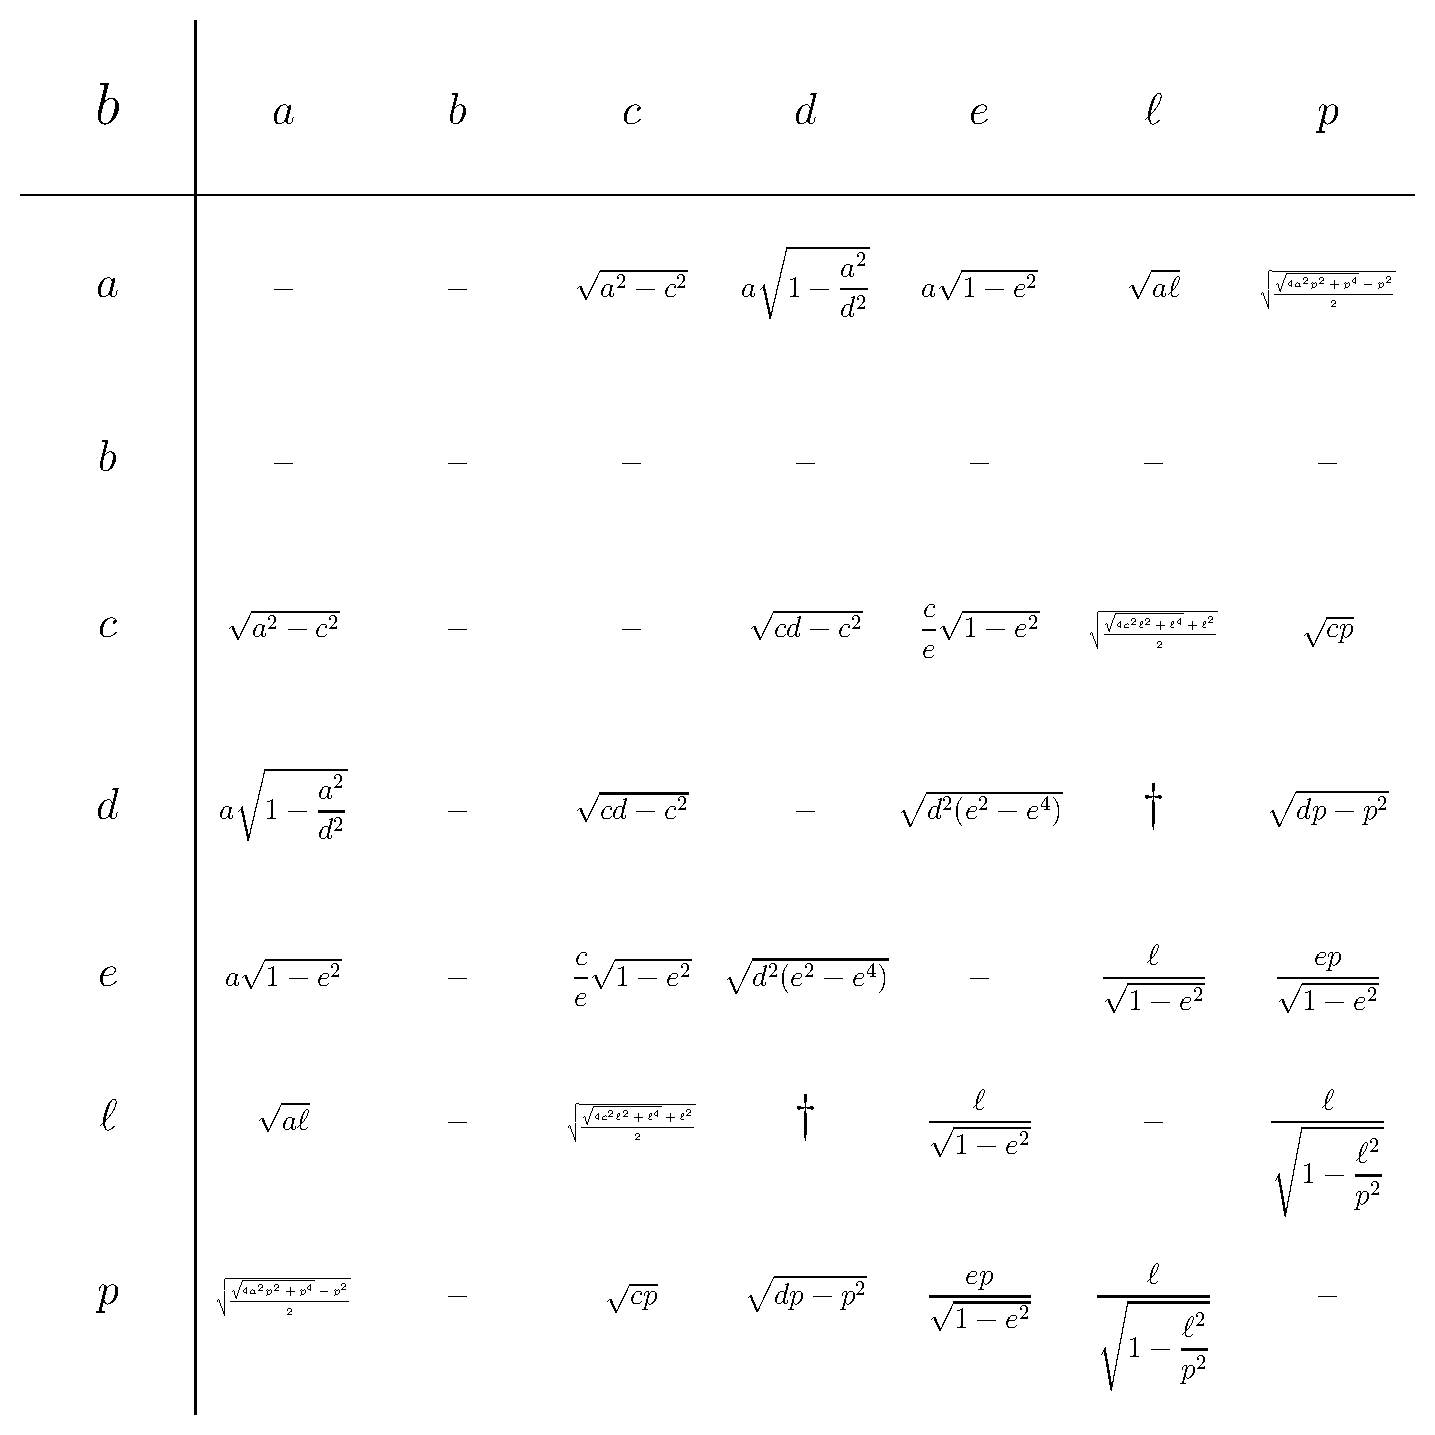
\includegraphics[scale=.95]{./BEquation/BEllipseEquations.pdf}
}
\newpage

\section*{\centering{Linear Eccentricity}}
\noindent\makebox[\textwidth]{%
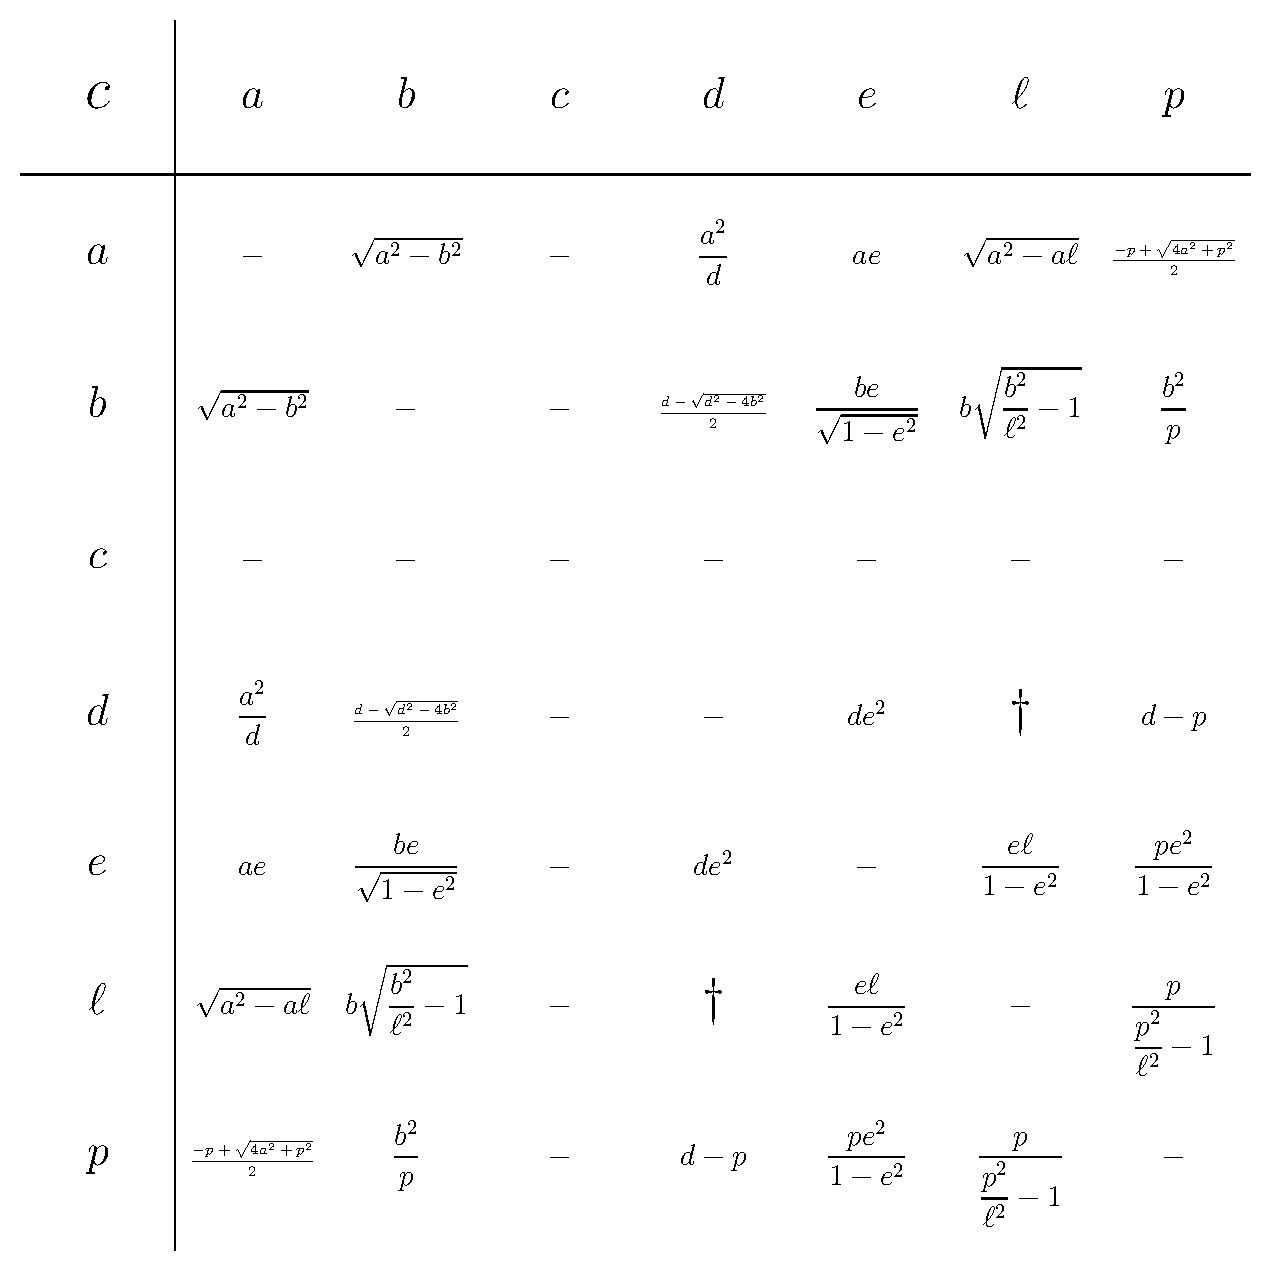
\includegraphics[scale=.95]{./CEquation/CEllipseEquations.pdf}
}
\newpage

\section*{\centering{Eccentricity}}
\noindent\makebox[\textwidth]{%
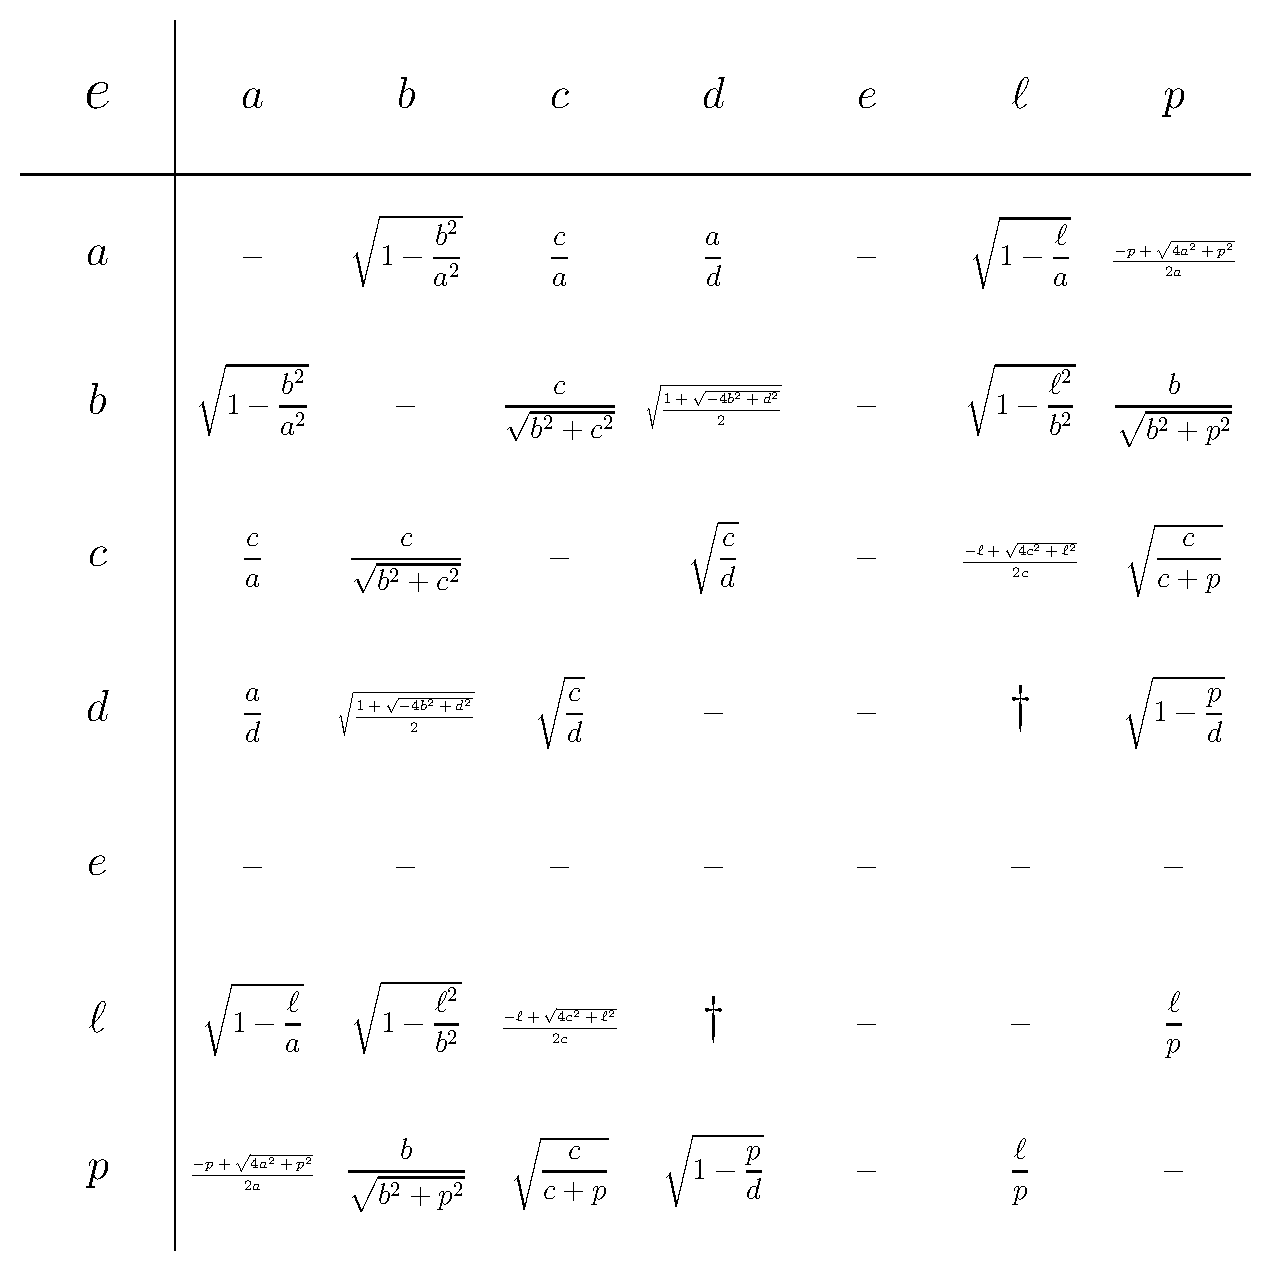
\includegraphics[scale=.95]{./EEquation/EEllipseEquations.pdf}
}
\newpage

\section*{\centering{Semi-Latus Rectum}}
\noindent\makebox[\textwidth]{%
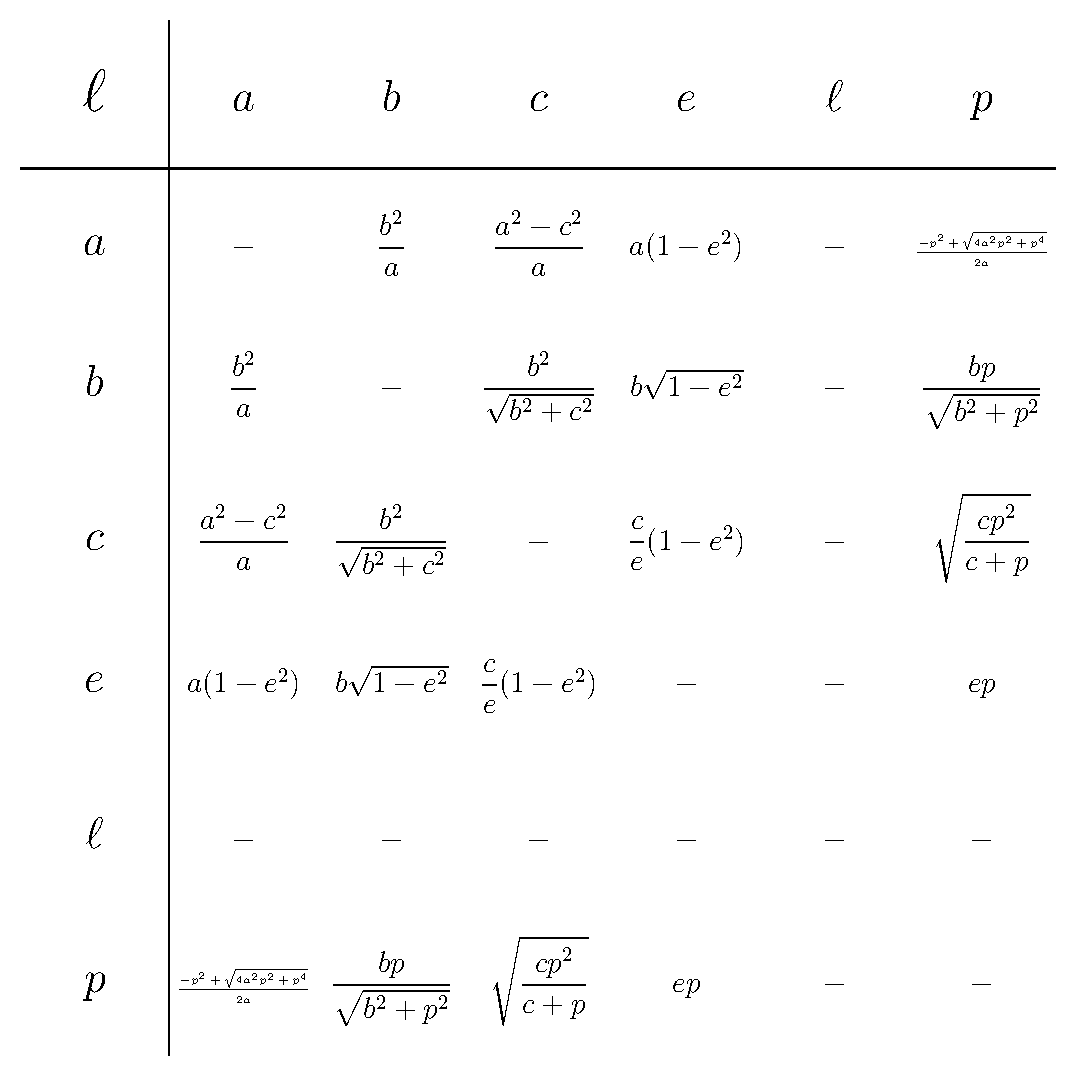
\includegraphics[scale=.95]{./LEquation/LEllipseEquations.pdf}
}
\newpage

\section*{\centering{Focal Parameter}}
\noindent\makebox[\textwidth]{%
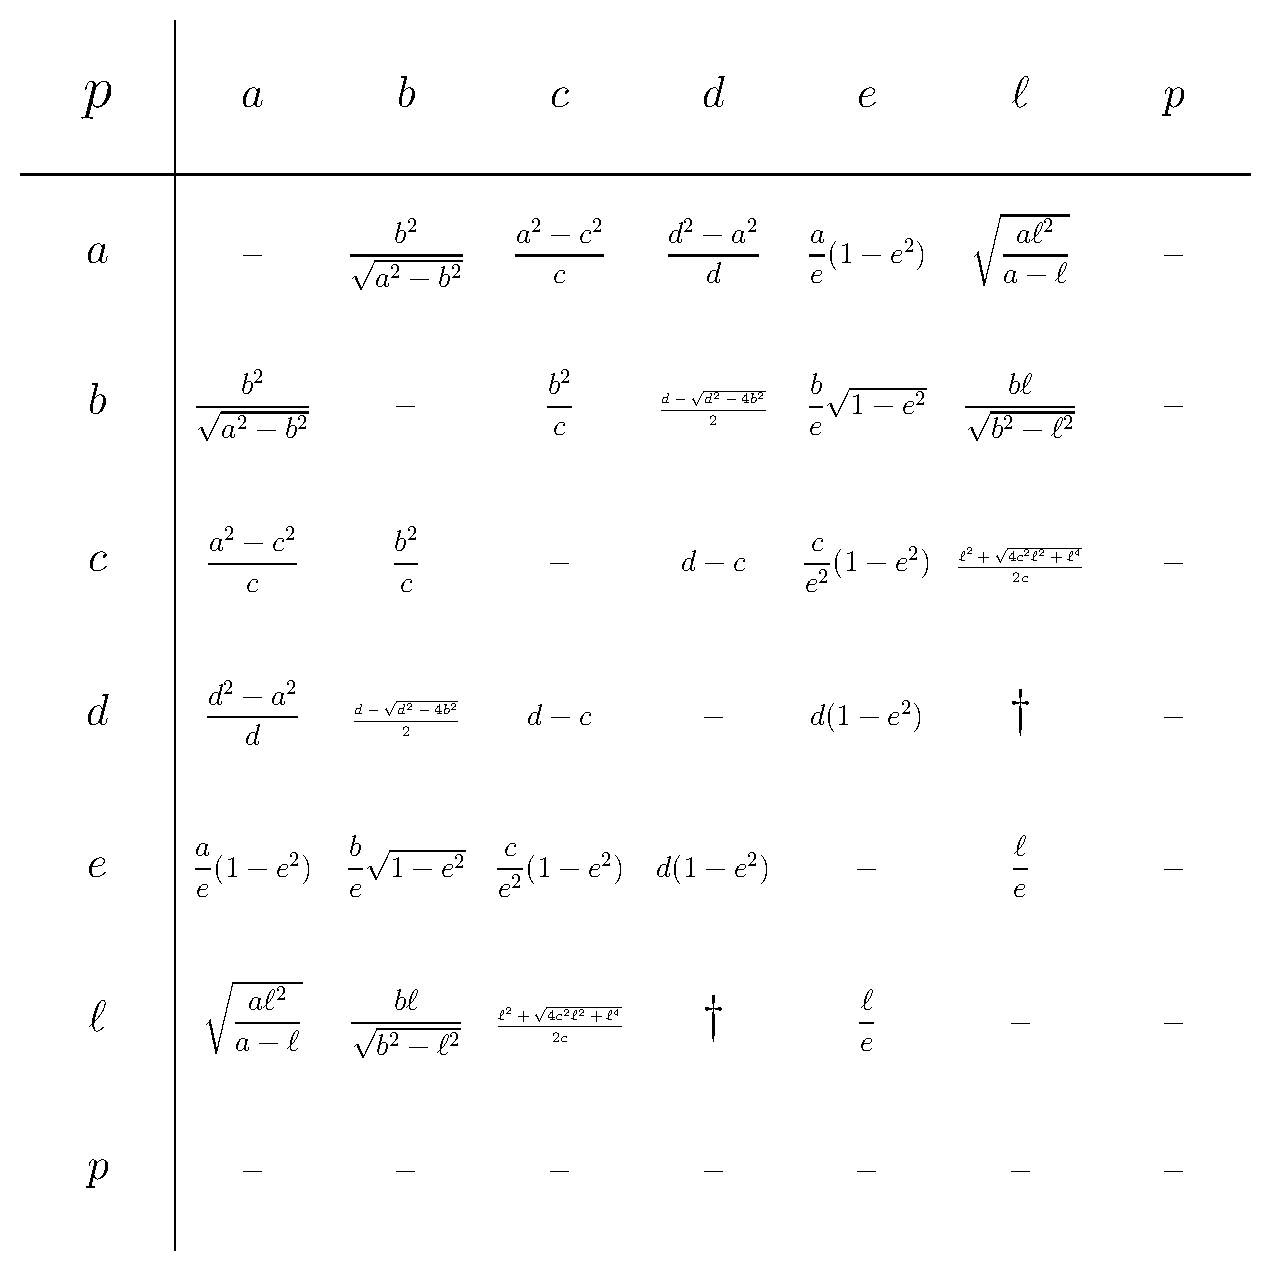
\includegraphics[scale=.95]{./PEquation/PEllipseEquations.pdf}
}

\section*{\centering{Directrix}}
\noindent\makebox[\textwidth]{%
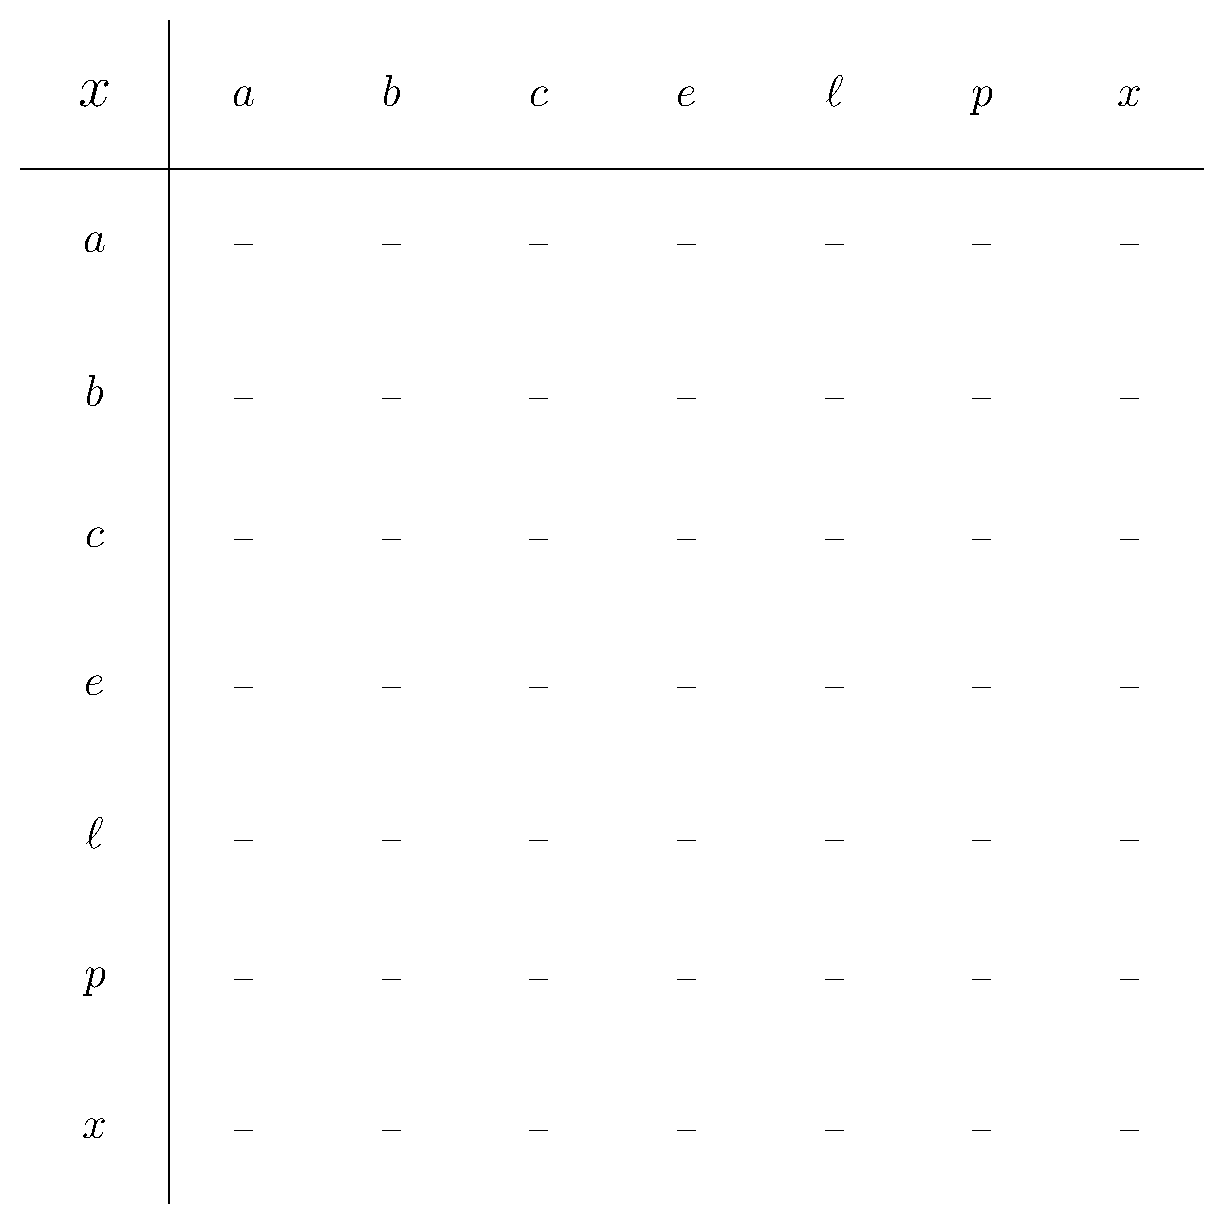
\includegraphics[scale=.95]{./XEquation/XEllipseEquations.pdf}
}
\end{center}
\end{document}